\documentclass[12pt]{article}
\usepackage{fullpage}
\usepackage[margin=0.5in]{geometry}
\usepackage{wrapfig}
\usepackage{graphicx}
\usepackage{url}
\usepackage{nopageno}

\setlength{\parindent}{0in}
\setlength{\parskip}{.2in}

\begin{document}

\begin{center}
\fbox{
\begin{minipage}{7.5in}
\centerline{\Huge The 30th Annual CCSC Eastern Regional Conference}

\centerline{\Large\it Catchy slogan}

\vskip .05in
\centerline{\bf November 14th and 15th, 2014: York College of Pennsylvania, York, Pennsylvania}

\vskip .1in
\centerline{\it Presented by the Consortium for Computing Sciences in Colleges}

\centerline{\it and the Computer Science and Computer Engineering Programs, York College of Pennsylvania}
\end{minipage}
}
\end{center}

\vskip -.1in
\begin{wrapfigure}[11]{r}{3in}
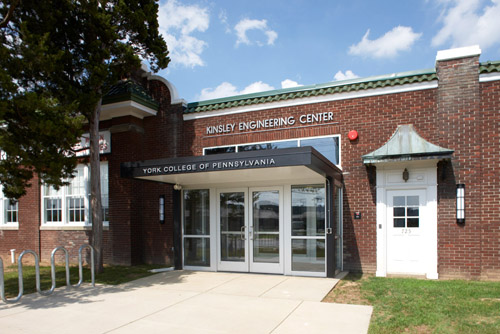
\includegraphics[width=3in]{kec}
\centerline{\it The Kinsley Engineering Center}
\end{wrapfigure}

The 30th Annual CCSC Eastern Regional Conference will be held on the campus
of York College of Pennsylvania.

Some shiznat about York College and its campus.

The 2013 CCSC Eastern Conference is designed to promote the exchange of information among
educators at all levels of the computing sciences. The conference spans all computing disciplines,
including computer science, computational science, information systems, information technology, and
beyond; and provides an affordable regional forum for the exchange of ideas and information
concerning computing and computing curricula.

The CCSC Eastern Conference welcomes scholarly papers, presentations, workshops, posters, and
panels on all areas of computing. We especially invite submissions that are of interest to
undergraduate students and submissions on the content, structure, delivery, support, and application
context of all areas of computing education.

There will be pre- and post-conference workshops, invited speakers, tutorials, panels,
lightning talks, and many sessions for papers. Two exciting activities are planned
for students: (a) a student poster session where undergraduate and graduate students
will have the opportunity to present research projects on any topic of the computing
sciences; and (b) a student team programming competition.
Both the student poster session and programming competition will award prizes.

Connecting with this yearʼs theme, {\em whatever our theme is}, we especially
welcome and encourage submissions related to all facets of {\em stuff related
to our theme}.

\begin{tabular}{ll}
{\bf Conference co-chairs}: & David Babcock (York College of Pennsylvania, dbabcock@ycp.edu) \\
                            & David Hovemeyer (York College of Pennsylvania, dhovemey@ycp.edu) \\
                            & Greg Link (York College of Pennsylvania, glink@ycp.edu) \\
                            & James Moscola (York College of Pennsylvania, jmoscola@ycp.edu) \\
{\bf Conference website}:   & \url{http://www.ccsc-eastern.org} \\
{\bf Submission deadline}:  & April 11, 2014

\end{tabular}

\end{document}
